%!TEX encoding = UTF-8 Unicode
%
% Laboratorio di Fisica III
% Esperienza 11
% Anno accademico 2013/2014
% Daniele Brugnara, Alessandro Casalino
%

\documentclass {article}
\usepackage[utf8]{inputenc}
\usepackage{fontenc}
\usepackage[italian]{babel}
\usepackage{graphicx}
\usepackage{float}
\usepackage{fancyhdr}
\usepackage{amsfonts}
\usepackage{amsmath}
\usepackage{amssymb}	
\usepackage{wrapfig}
\usepackage{enumitem}
\usepackage{subfigure}
\usepackage{siunitx}
\usepackage{footnote}
\usepackage [a4paper, top=1.8cm, bottom=2cm, left=0.9cm, right=0.9cm] {geometry}
\pagestyle{fancy}

\makeatletter
\@addtoreset{section}{part}
\makeatother
\rhead{\LARGE Quaderno di Laboratorio}

\lhead{\large Laboratorio di Fisica IV}
\lfoot{GruppoA10 - A. Casalino}
\cfoot{}
\rfoot{\thepage}
\renewcommand{\headrulewidth}{0.7pt}
\renewcommand{\footrulewidth}{0.7pt}

\begin {document}

\begin{titlepage}
\begin{center}


\includegraphics[width=0.3\textwidth]{unitn_logo.jpg}~\\[1cm]

\textsc{\LARGE Laboratorio di Fisica IV}\\[1.5cm]
\textsc{\Large Gruppo A10}\\[0.5cm]

{ \huge \bfseries Quaderno di Laboratorio}\\[0.4cm]

\begin{minipage}{0.4\textwidth}
\begin{flushleft} \large
\emph{}\\
\centerline {\large Casalino Alessandro}
\end{flushleft}
\end{minipage}

\vfill

{\large}

\end{center}
\end{titlepage}
\part*{16.09.2014 - Amplificatori Operazionali Ideali}

\section{Introduzione}

In questa sessione di laboratorio abbiamo montato due circuiti con amplificatori operazionali: un generatore di corrente costante e un sommatore pesato. Nel primo caso abbiamo controllato se la corrente rimanesse costante al variare della resistenza di carico; nel secondo caso abbiamo valutato la tensione di uscita.

\section{Materiali}

\begin{itemize} [noitemsep]
\item Oscilloscopio Agilent DSO-X 2002A (bandwidth $70$ \si{\mega\hertz}, sample rate $2$ GSa/s);
\item Generatore di tensione continua Agilent E3631A (max $\pm 25$ \si{\volt} o $\pm 6$ \si{\volt});
\item Generatore di tensione Agilent 33120A con range di frequenza da $100$ \si{\micro\hertz} a $15$ \si{\mega\hertz};
\item Multimetro Agilent 34410A (utilizzato come amperometro e per verificare i valori delle resistenze);
\item Un amplificatore operazionale UA741;
\item Resistenze di vari valori;
\item Due capacità da $0.1$ \si{\micro\farad} (i valori misurati sono in Figura \ref{gr:costante});
\item Breadboard e cablaggi vari.
\end{itemize}

\section{Premessa sugli amplificatori operazionali ideali}

Durante l'esperienza valuteremo l'amplificatore operazionale considerandolo come ideale. Infatti, in questa approssimazione (peraltro non eccessivamente limitante visti i valori di corrente in gioco nel nostro caso), valgono (considerando come A e B rispettivamente gli ingressi invertente e non invertente):

\begin{equation}
\Delta V_{AB}=0
\label{eq:regola_V}
\end{equation}
\begin{equation}
I_{AB}=0
\label{eq:regola_I}
\end{equation}

cioè la ddp fra l'ingresso invertente e non invertente è portato ad essere nullo dall'amplificatore operazionale modificando il valore di tensione in output (il cosiddetto \textit{ground virtuale} dato che nei nostri casi l'ingresso non invertente è collegato alla comune del circuito); e la corrente assorbita dall'amplificatore è nulla.
Queste regole verranno utilizzate durante questa sessione per valutare la risposta del circuito a segnali in ingresso, e si intendono utilizzate per tutte le sessioni in cui l'amplificatore è considerato ideale.

\begin{figure}[ht]
 \centering
   {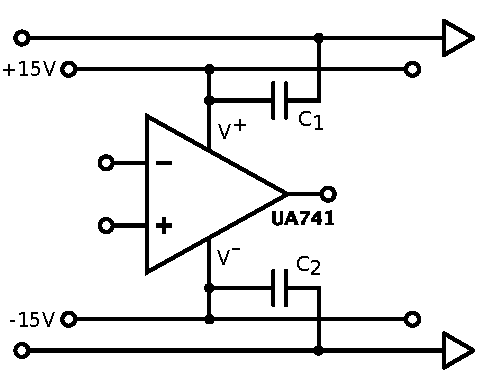
\includegraphics[width=6cm]{../E01/latex/alimentazione.pdf}}
 \caption{Grafico dell'alimentazione dell'OPAMP. La tensione di alimentazione è fornita con il generatore di tensione costante, mentre le capacità sono $C_1=(0.112 \pm 0.001)$ \si{\micro\farad} $C_2=(0.095\pm0.001)$ \si{\micro\farad}. Per maggiore chiarezza negli schemi circuitali, questa configurazione sarà nascosta negli schemi successivi, ma comunque presente sulla breadboard.}
 \label{gr:costante}
\end{figure}

Inoltre, al fine di evitare problemi di rumore durante l'alimentazione, abbiamo collegato l'alimentazione a due capacità come nello schema in Figura \ref{gr:costante}.

\section{Generatore di corrente}

In questo circuito abbiamo assemblato un generatore di corrente costante, cioè un dispositivo in grado di erogare una corrente costante ai capi di una resistenza (che definiremo \textit{resistenza di carico} $R_c$), indipendentemente dal valore di quest'ultima. Per valutare questa caratteristica abbiamo dunque utilizzato come $R_c=R_2$ una resistenza variabile di tipo \textit{trimmer}. Lo schema circuitale è in Figura \ref{gen_continua}.

\begin{wrapfigure}[21]{r}{0.55\textwidth}
  \begin{center}
    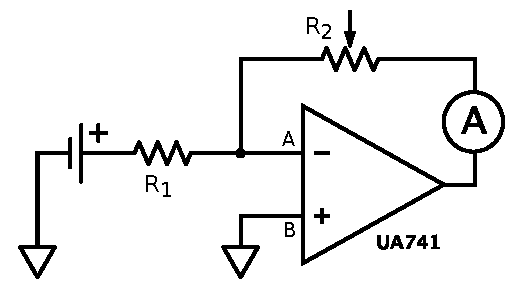
\includegraphics[width=0.40\textwidth]{../E01/latex/c1.pdf}
  \end{center}
  \caption{Schema del generatore di corrente costante. Come valori abbiamo utilizzato $R1=(3.85 \pm 0.01)$ \si{\kilo\ohm} e $V_{gen}=3.85$ \si{\volt}, mentre $R_2$ è variabile. Come amperometro è utilizzato il multimetro, mentre per alimentare l'OPAMP e come generatore di tensione costante in figura, abbiamo utillizzato il generatore Agilent E3631A.}
  \label{gen_continua}
\end{wrapfigure}

Risolviamo ora il circuito, considerando la tensione fornita dal generatore di tensione continua come $V_{gen}$ e la tensione in uscita dall'OPAMP come $V_{out}$. Dato che B si trova a potenziale di comune, per (\ref{eq:regola_V}) anche A sarà allo stesso potenziale, che considereremo nullo. Dunque varranno
\begin{equation}
V_{gen} - V_A = V_{gen} = I_1 R_1
\label{eq:gen_1}
\end{equation}
$$V_A-V_{out} = -V_{out} = I_2 R_2$$
Per (\ref{eq:regola_I}) e la legge di Kirkhhoff sui nodi, avremo invece che la corrente passante per la resistenza di carico è uguale alla corrente di (\ref{eq:gen_1}). Dunque $I=I_1=I_2$.

Otteniamo dunque che la tensione di output si modificherà, ad opera dell'OPAMP, in modo da far passare sempre lo stesso valore di corrente attraverso $R_2$; ciò avviene per il fenomeno di retroazione negativa, che ci permette di controllare la tensione di output tramite la resistenza di feedback, che in questo caso è $R_2$, e di ottenere dunque una corrente costante passante per il circuito di feedback. Imponendo l'uguaglianza della corrente possiamo inoltre trovare il valore della tensione di uscita

$$V_{out}=-\frac{R_2}{R_1} V_{gen}$$

Durante l'esperienza abbiamo però deciso di misurare la corrente passante per la resistenza piuttosto che la tensione di uscita, ponendo un amperometro fra l'uscita dell'OPAMP e la resistenza di carico $R_2$. Come valore di corrente abbiamo scelto $1$ \si{\milli\ampere}, discostandoci dalla corrente massima in cui l'amplificatore operazionale potrebbe non comportarsi più in maniera ideale ($10/20$ \si{\milli\ampere}); e avendo a disposizione una resistenza $R_1=(3.85 \pm 0.01)$ \si{\kilo\ohm}, per (\ref{eq:gen_1}), abbiamo utilizzato una tensione continua di $3.85$ \si{\volt}. Di seguito proponiamo alcuni valori sperimentali che confermano la capacità del circuito da noi creato di fornire alla resistenza di carico una corrente costante di $1$ \si{\milli\ampere}.

\begin{center}
\begin{tabular}{c|c|c|c|c|c|c|c|c}
Resistenza variabile [\si{\ohm}] & 0.54 & 35.1 & 412 & 1021 & 1996 & 3068 & 4170 & 4719 \\ 
\hline 
Corrente nel carico [\si{\milli\ampere}] & 1.002 & 1.002 & 1.002 & 1.002 & 1.002 & 1.002 & 1.002 & 1.002 \\ 
\end{tabular}
\end{center}

Gli errori sulla tabella sono uguali, cioè unitari sull'ultima cifra del valore, sia per le resistenza che per le correnti.

\section{Sommatore Pesato}

\subsection{Circuito}

Valutiamo ora il sommatore pesato, cioè un circuito che dati alcuni segnali in ingresso (due nel nostro caso) li somma con relativi pesi dati dal rapporto fra la resistenza di feedback ($R_f$) e quella a loro associata ($R_1$ e $R_2$). Lo schema circuitale è in Figura \ref{sommatore_pesato}.

\begin{wrapfigure}[21]{l}{0.55\textwidth}
  \begin{center}
    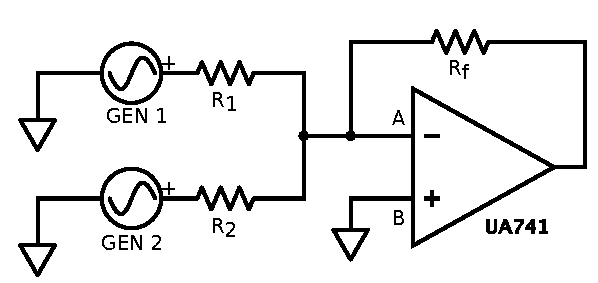
\includegraphics[width=0.40\textwidth]{../E01/latex/c2.pdf}
  \end{center}
  \caption{Schema del sommatore pesato. Come valori abbiamo utilizzato $R_f=(99.7 \pm 0.1)$ \si{\kilo\ohm}, $R_1=(99.9 \pm 0.1)$ \si{\kilo\ohm} e $R_2=(49.8 \pm 0.1)$ \si{\kilo\ohm}, dove per $R_2$ è stato necessario utilizzare un parallelo di due resistenza da $100$ \si{\kilo\ohm}. Come GEN 1 abbiamo utilizzato l'oscilloscopio, mentre per GEN 2 il generatore di forme d'onda. Infine, per valutare la tensione in uscita abbiamo utilizzato l'oscilloscopio.}
  \label{sommatore_pesato}
\end{wrapfigure}

Per risolvere il circuito consideriamo, definendo le tensioni dei generatori 1 e 2 rispettivamente $V_1$ e $V_2$, le seguenti equazioni derivanti dalle leggi di Kirkhhoff e dalla (\ref{eq:regola_I})
$$V_1 - V_A =I_1 R_1 \qquad V_2 - V_A =I_2 R_2$$
$$V_A - V_{out} =(I_1+I_2) R_f$$
Per (\ref{eq:regola_V}) vale inoltre che $V_A=V_B=0$; dunque otteniamo, sostituendo le correnti nell'ultima equazione sopra
$$V_{out}=-R_f \left( \frac{V_1}{R_1}+\frac{V_2}{R_2}\right)$$

Si può dunque definire un peso relativo $\phi_i$ ad ogni segnale dato dal rapporto fra $R_f$ ed $R_{i}$ (con $i=1,2$) e scrivere una formula del tipo
$$V_{out}=-\sum^{2}_{i=1} \frac{R_f}{R_{i}}V_{i}=-\sum^{2}_{i=1} \phi_i V_{i}$$

Durante l'esperienza abbiamo optato per valori semplici dei rapporti fra le resistenze, utilizzando i seguenti valori: $R_f=R_1=100 k\Omega$ e $R_2=50 k\Omega$. Si ottengono dunque $\phi_1=1$ e $\phi_2=2$.

\subsection{Grafici}

Presentiamo ora i grafici di alcune forme d'onda in uscita.

$$$$

\begin{figure}[ht]
 \centering
   {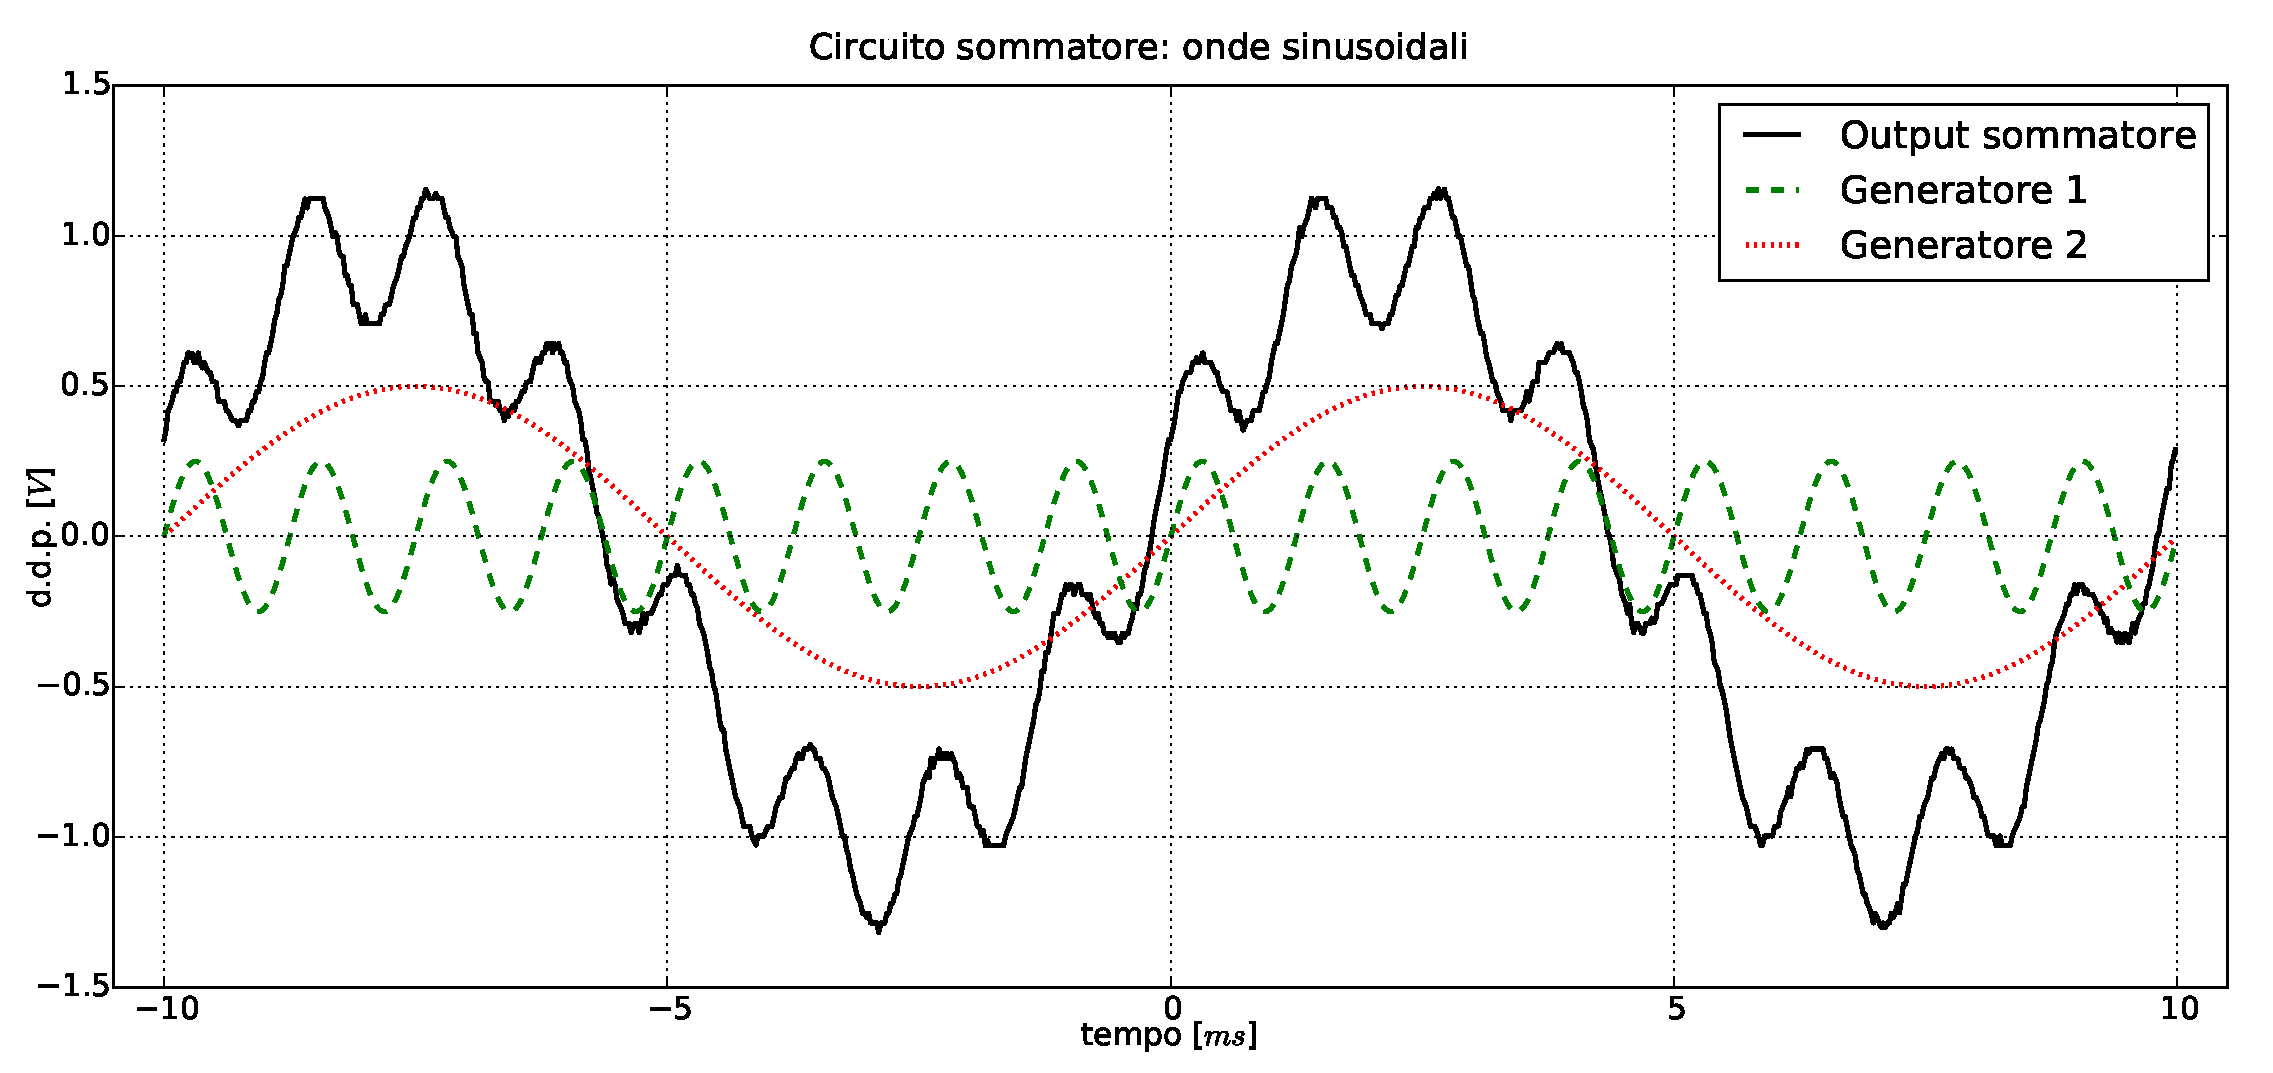
\includegraphics[width=16.5cm]{../E01/latex/sinsin.pdf}}
 \caption{Grafico della tensione di uscita. Il generatore 1 (generatore dell'oscilloscopio) crea un'onda sinusoidale di $\nu=800$ \si{\hertz} e $V^1_{pp}=500$ \si{\milli\volt}; il generatore 2 (generatore di forme d'onda) crea invece un'onda sinusoidale di $\nu=100$ \si{\hertz} e $V^2_{pp}=1000$ \si{\milli\volt}. Notiamo inoltre che l'ampiezza massima è pari a $\phi_1 V^1_{pp}+\phi_2 V^2_{pp}=2500$ \si{\milli\volt}.}
 \label{gr:onde1}
\end{figure}

$$$$

\begin{figure}[ht]
 \centering
   {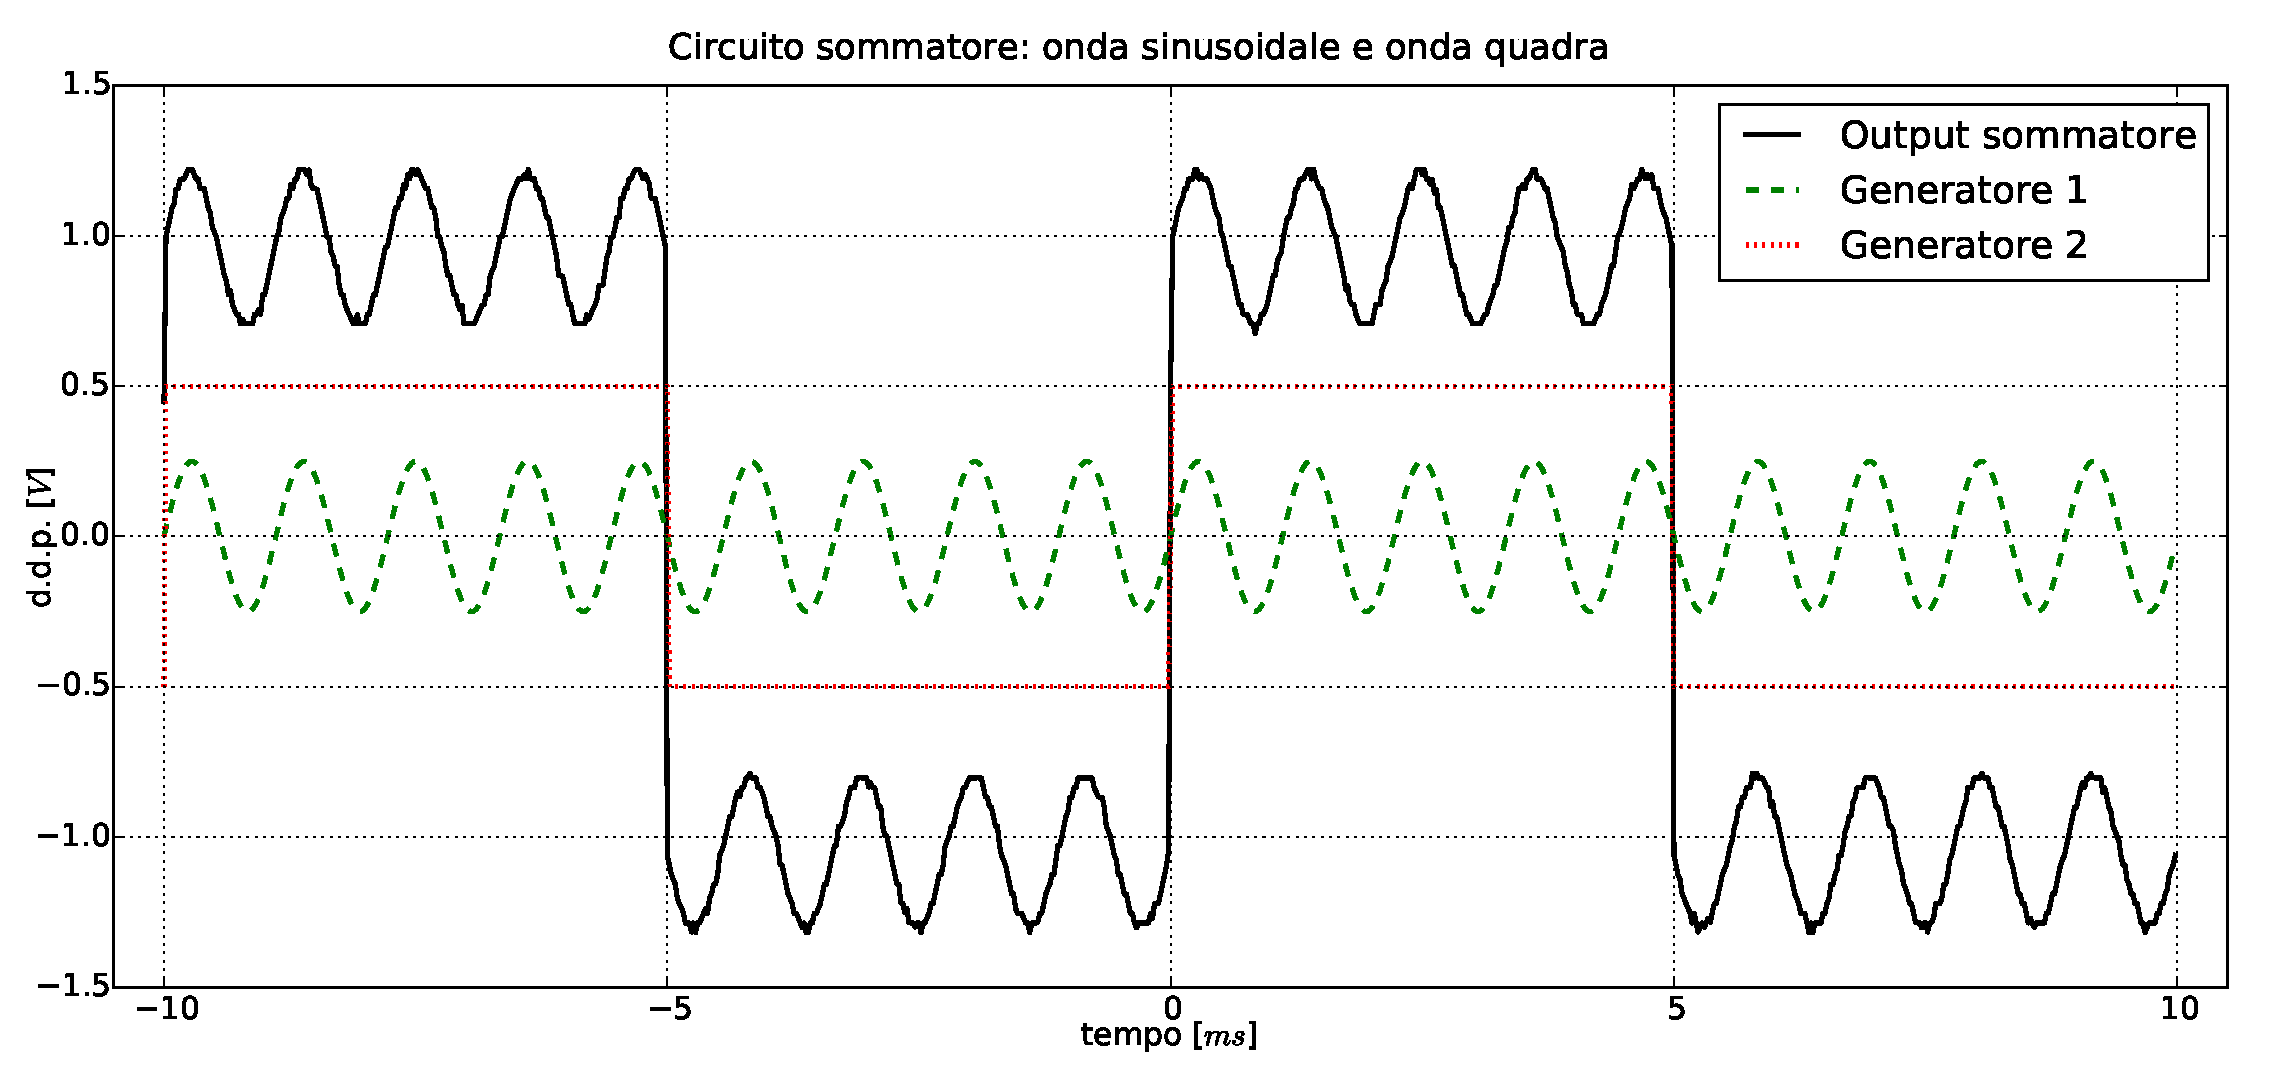
\includegraphics[width=16.5cm]{../E01/latex/sinquad.pdf}}
 \caption{Grafico della tensione di uscita. Il generatore 1 (generatore dell'oscilloscopio) crea un'onda sinusoidale di $\nu=900$ \si{\hertz} e $V^1_{pp}=500$ \si{\milli\volt}; il generatore 2 (generatore di forme d'onda) crea invece un'onda quadra di $\nu=100$ \si{\hertz} e $V^2_{pp}=1000$ \si{\milli\volt}. Notiamo inoltre che anche in questo caso l'ampiezza massima è pari a $\phi_1 V^1_{pp}+\phi_2 V^2_{pp}=2500$ \si{\milli\volt}.}
 \label{gr:onde2}
\end{figure}

\subsection{Battimenti}

Utilizzando due forme d'onda sinusoidali con il sommatore, abbiamo potuto il battimento, fenomeno che si verifica quando la differenza fra le frequenze delle onde in ingresso è sufficientemente bassa.

Con due onde abbiamo che:
$$V_{out}=\phi_1 A_1 \sin [2 \pi \nu_1 t + \theta_1] + \phi_2 A_2 \sin [2 \pi \nu_2 t + \theta_2]$$

Supponiamo che $A=\phi_1 A_1=\phi_2 A_2$, come nel caso del grafico sotto riportato. Utilizzando le formule di prostaferesi otteniamo che

$$V_{out}=2A \sin \left[4 \pi (\nu_1 + \nu_2) t + \frac{\theta_1+\theta_2}{2}\right] \cos \left[4 \pi (\nu_1 - \nu_2)t + \frac{\theta 1-\theta_2}{2}\right]$$


\begin{figure}[ht]
 \centering
   {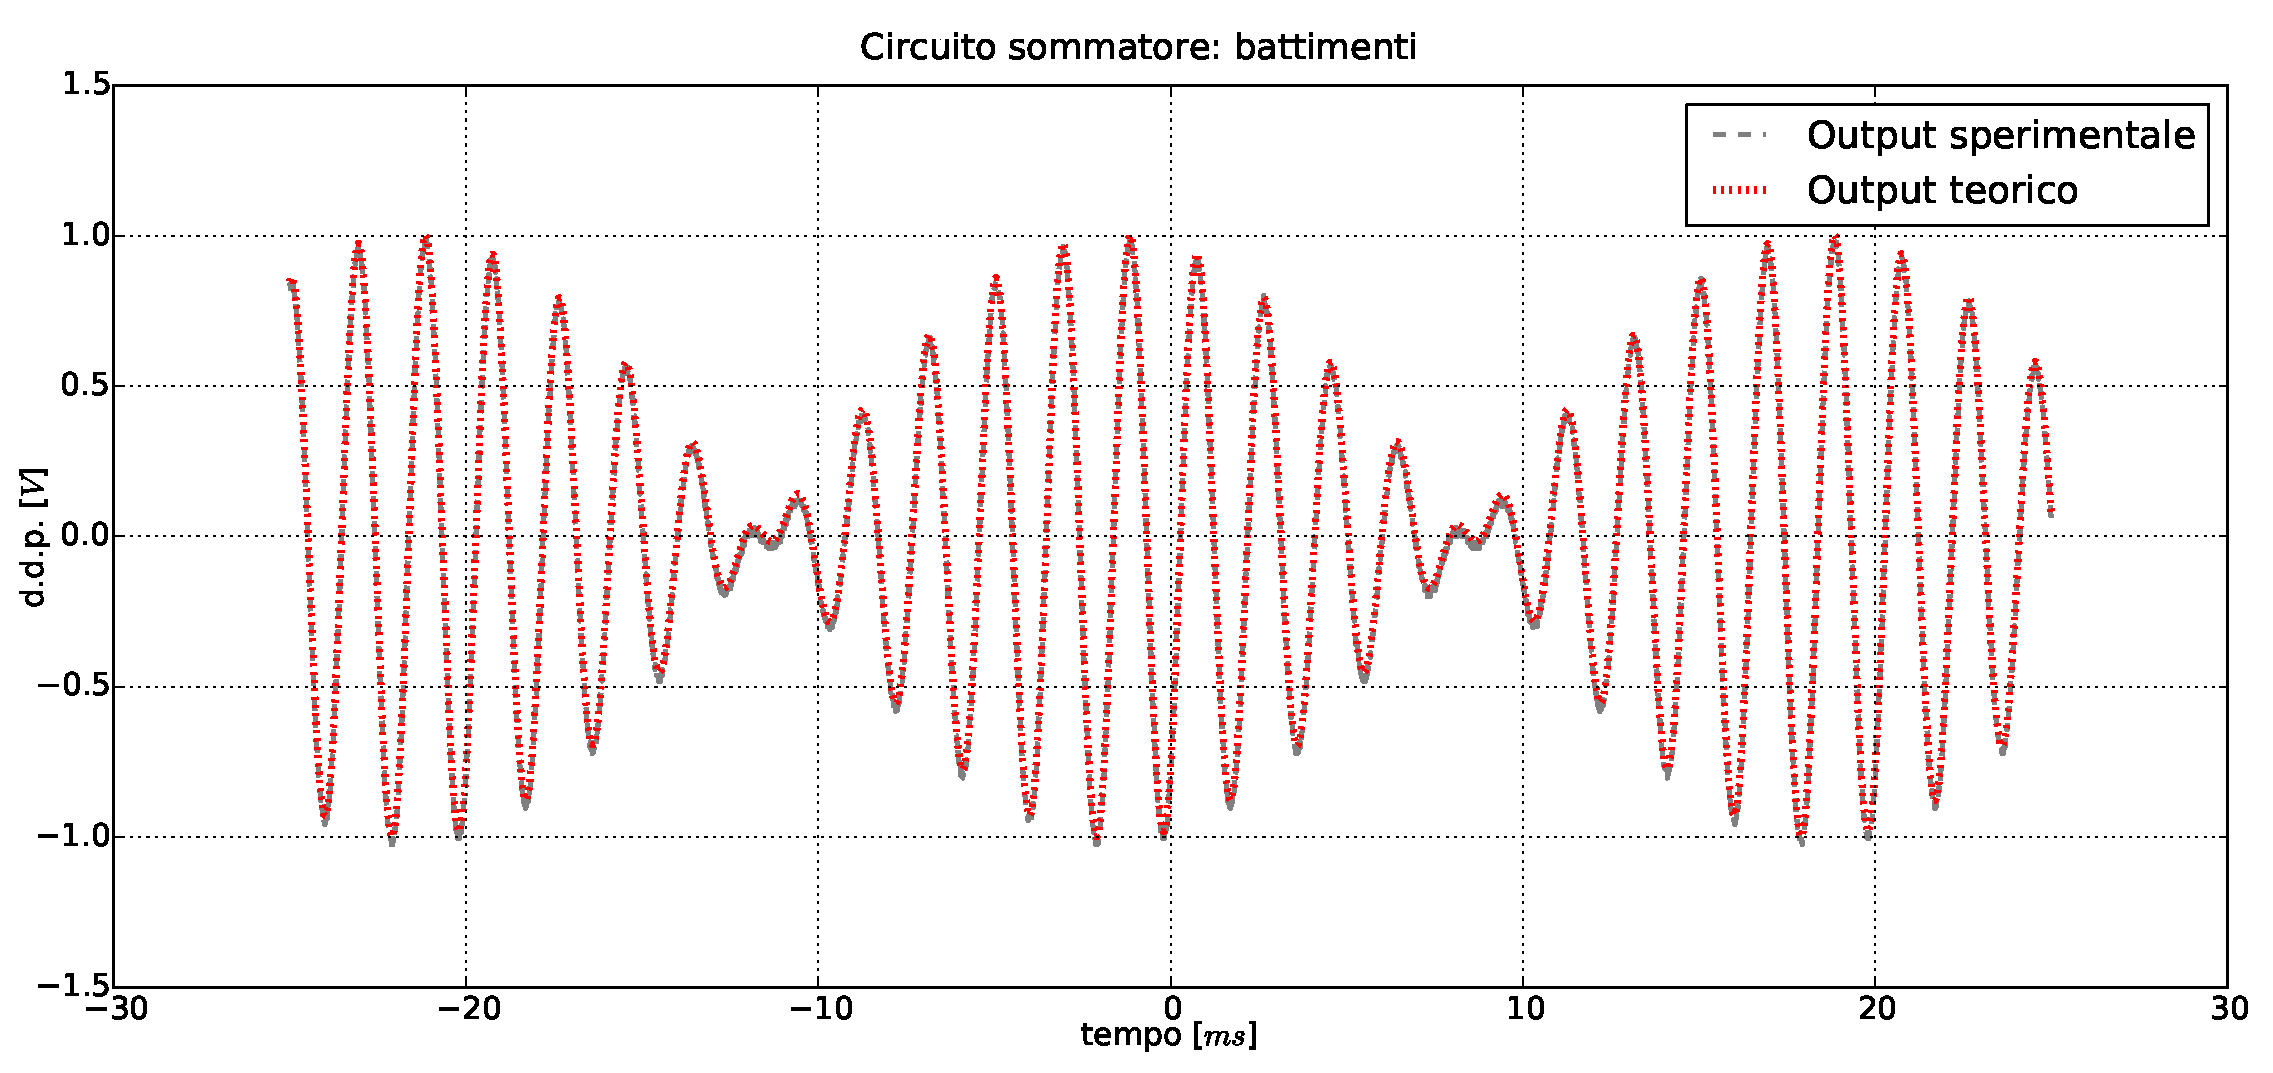
\includegraphics[width=17.5cm]{../E01/latex/battimenti_ideali.pdf}}
 \caption{Grafico della tensione di uscita. Il generatore 1 (generatore dell'oscilloscopio) crea un'onda sinusoidale di $\nu=900$ \si{\hertz} e $V^1_{pp}=500$ \si{\milli\volt}; il generatore 2 (generatore di forme d'onda) crea invece un'onda quadra di $\nu=100$ \si{\hertz} e $V^2_{pp}=1000$ \si{\milli\volt}. Notiamo inoltre che anche in questo caso l'ampiezza massima è pari a $\phi_1 V^1_{pp}+\phi_2 V^2_{pp}=2500$ \si{\milli\volt}.}
 \label{gr:battimenti}
\end{figure}

\newpage

\setcounter{section}{0}
\setcounter{figure}{0}
\setcounter{equation}{0}

\section{Titolo - 24.09.2014}

\subsection{Strumenti e materiali}

\begin{itemize} [noitemsep]
\item Oscilloscopio Agilent DSO-X 2002A (bandwidth \SI{70}{\mega\hertz}, sample rate \num{2} GSa/s);
\item Generatore di tensione continua Agilent E3631A (max $\pm \, \SI{25}{\volt}$ o $\pm \, \SI{6}{\volt}$);
\item Generatore di forme d'onta Agilent 33120A con range di frequenza da \SI{100}{\micro\hertz} a \SI{15}{\mega\hertz};
\item Multimetro Agilent 34410A;
\item Un amplificatore operazionale $\mu$A741;
\item Resistenze di vari valori;
\item Due capacità da \SI{0.1}{\micro\farad};
\item un trimmer (potenziometro);
\item Breadboard e cablaggi vari.
\end{itemize}

\subsection{Stima e correzione dell'offset}
\label{par2:offset}

In questa prima parte dell'esperienza tratteremo il problema dell'offset. In un amplificatore ideale sappiamo che quando sia ingresso invertente che ingresso non invertente sono collegati a comune il segnale in uscita è nullo. Ciò è dovuto alla perfetta simmetria interna dell'op-amp. Ovviamente nel mondo reale non è possibile realizzare tale fatto in quanto non si riescono a costruire transistor BJT con specifiche identiche. 

\subsubsection{Configurazione senza retroazione}

Quando colleghiamo entrambi gli ingressi a comune l'op-amp vede all'ingresso una differenza di potenziale (ovviamente, fra gli ingressi non c'è, in quanto collegati entrambi a comune) la quale viene amplificata dal guadagno a maglia aperta: come $V_{out}$ avremo dunque un valore diverso da zero. Nel nostro caso l'op-amp andava in saturazione negativa (\SI{-12.9}{\volt}). Ricordando il funzionamento di un amplificatore operazionale, possiamo dire che il circuito si comporta come se la tensione all'ingresso invertente fosse maggiore di quella all'ingresso non invertente. Inoltre il valore $V_{out}$ è diverso da \SI{-15}{\volt} utilizzati come alimentazione in quanto il valore di tensione massimo $|V_{out}|$ è leggermente inferiore a $|V^-|$. In Figura(\ref{cir:open_loop}) è riportato lo schema del circuito utilizzato.

\begin{figure}[ht]
        \centering
        \begin{subfigure}[b]{0.35\textwidth}
                 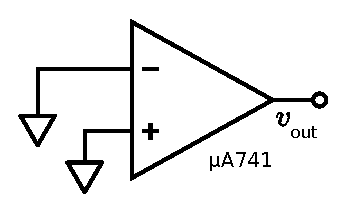
\includegraphics[width=0.70\textwidth]{../E02/latex/open_loop.pdf}
                \caption{Circuito a maglia aperta}
                \label{cir:open_loop}
        \end{subfigure}%
    \quad
        \begin{subfigure}[b]{0.35\textwidth}
               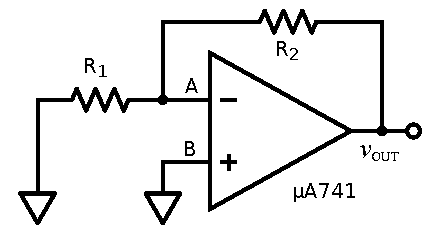
\includegraphics[width=0.70\textwidth]{../E02/latex/inv.pdf}
                \caption{Circuito amplificatore}
                \label{cir:inv}
        \end{subfigure}
     
\end{figure}

Con il circuito in Figura (\ref{cir:open_loop}) non possiamo quindi ricavare una stima del valore di offset. Per fare ciò dobbiamo ricorrere a un circuito amplificatore come quello in Figura(\ref{cir:inv}) (invertente o non invertente), che ci permetta di controllare il guadagno.

\subsubsection{Configurazione con retroazione}

Trattiamo per primo il caso \textbf{invertente}. Assumiamo che la tensione nel punto A sia $V_A=V_{off}$ e $V_B=0$. L'analisi del circuito è ora banale e risulta immediatamente $V_{out}=-\frac{R_2}{R_1}V_{off}$. Ovviamente, visto che il punto A è collegato al comune, la sua tensione sarà identica a quella del punto A. La tensione $V_{off}$ è infatti un valore che concerne la struttura stessa dell'op-amp. Assumere che il punto A sia alla tensione $V_{off}$ permette dunque di analizzare il circuito. 

Ora analogamente tratteremo il caso \textbf{non invertente}. Per far ciò assumiamo $V_B=-V_{off}$ e $V_A=0$. L'analisi risulta dunque identica a quella di un amplificatore non invertente, ovvero $V_{out}=(1+\frac{R_2}{R_1})V_{off}$. 

%I valori nominali delle componenti circuitali utilizzate sono: $R_1=\SI{120}{\ohm}$ e $R_2=\SI{10/100}{\kilo\ohm}$.

Riportiamo nella seguente tabella i valori di offset calcolati nei due casi:

\begin{center}
\begin{savenotes}
\begin{tabular}{c|c|c|c|c|c|c}
$R_1[\si{\ohm}]$ & $R_2[\si{\kilo\ohm}]$ & Gain(inv) & Gain (ninv) &$V_{out} [\si{\milli\volt}]$ & $V_{off}$(inv)[\si{\milli\volt}] &$V_{off}$(ninv) [\si{\milli\volt}]\\ 
\hline 
$119.8\pm0.1$ & $9.911\pm0.001$  & $-82.73\pm0.07$ &$83.73\pm0.07$&  $-103.5 \pm 0.5$ & $-1.251 \pm0.006$ & $-1.23 \pm0.01$\\
\hline
$119.8\pm0.1$ & $99.35\pm0.01$  & $-829.3\pm0.7$ & $830.3\pm0.7$ &$ -1025 \pm 2$ & $-1.236 \pm 0.002$ & $-1.2 \pm0.1$\\

\end{tabular}
\end{savenotes}
\end{center}

Ricordiamo che i valori di tensione di offset ottenuti per configurazione invertente e non invertente differiscono nel segno in quanto è necessario che in entrambi i casi sia rispettata la condizione $|V_{inv}|>|V_{ninv}|$.

Come sappiamo la tensione di offset non è però l'unico problema che incontriamo quando usiamo op-amp reali. Infatti ingresso invertente e non invertente sono collegati alle basi di transistor e, ovviamente, per polarizzarli serve una corrente di base. Gli effetti di tale corrente si sommeranno dunque a quelli dovuti all'offset. Tale argomento sarà comunque trattato approfonditamente nella sezione successiva. Per risolvere il problema dell'offset possiamo servirci di una resistenza variabile ($trimmer$) che posizioneremo tra i piedini 1 e 5 dell'op-amp, collegandola a $V^-$. Regolando tale resistenza andremo a generare una contro tensione che bilancerà l'offset. 

\begin{wrapfigure}[17]{l}{0.55\textwidth}
  \begin{center}
    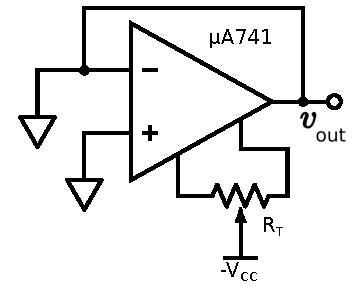
\includegraphics[width=0.260\textwidth]{../E02/latex/trimmer_correction.pdf}
  \end{center}
  \caption{Circuito con trimmer per compensare l'offset.}
  \label{cir2:trimmer}
\end{wrapfigure}

Il datasheet dell'amplificatore consiglia di utilizzare un circuito a maglia aperta senza resistenze per regolare il trimmer. Tale configurazione è consigliata sia per la simmetria dei due ingressi (entrambi vedono la stessa impedenza $\approx 0$) sia per il fatto che il guadagno a maglia aperta molto grande ci permette praticamente di azzerare l'offset. 

Durante l'esperienza abbiamo provato ad utilizzare trimmer ad un giro da \SI{10}{\kilo\ohm} ma la sensibilità meccanica era troppo bassa per poter azzerare l'offset (la tensione di uscita infatti passava da $\approx$\SI{-13}{\volt} a $\approx$\SI{+13}{\volt}). Abbiamo dunque utilizzato un trimmer multigiro da \SI{10}{\kilo\ohm}, con il quale abbiamo raggiunto la tensione $V_{out}= (1.3\pm0.2)\si{\volt}$. Ricordando che il guadagno a maglia aperta è di 100-120dB, si nota il buon bilanciamento della tensione di offset.

Come già accennato le correnti di bias, per quanto piccole (\si{\nano\ampere}) giocano comunque un ruolo non indifferente sull'offset totale. Se assumiamo che $I_B^- \simeq I_B^+ $, allora basterà fare in modo che i due ingressi vedano la stessa impedenza. Così facendo il contributo delle due correnti si bilancia e abbiamo una stima più precisa dell'offset. Abbiamo dunque ripetuto le misure. Riportiamo nella seguente tabella i nuovi valori:

\begin{tabular}{c|c|c|c|c|c|c}
$R_C [\si{\ohm}]$& $R_1[\si{\ohm}]$ & $R_2[\si{\kilo\ohm}]$ & Gain (inv) & $V_{out}' [\si{\milli\volt}]$ & $V_{off}' [\si{\milli\volt}]$ & $|V_{off}-V_{off}'|[\si{\milli\volt}]$ \\ 
\hline 
$119.4\pm0.1$ & $119.8\pm0.1$ & $9.911\pm0.001$  & $-82.73\pm0.07$ & $-105.5 \pm 0.5$ & $-1.275 \pm0.006$ & $0.024\pm0.008$ \\
\hline
$119.4\pm0.1$ & $119.8\pm0.1$ & $99.35\pm0.01$  & $-829.3\pm0.7$ &$ -1038 \pm 5$ & $-1.251 \pm 0.002$ & $0.015 \pm 0.003 $	\\

\end{tabular}

Come vediamo, le differenze tra i due valori di $V_{off}$ calcolati con e senza resistenza $R_C$ sono compatibili al contributo di una corrente $I^*$ dell'ordine dei \si{\nano\ampere} che scorre nella resistenza $R_C$: $\Delta V \simeq R_C * 10^{-9} \simeq 10\div100 \si{\micro\volt}$.

Anche nel caso non invertente $\Delta V$ risulta compatibile con la caduta di potenziale data da una corrente di base di alcuni \si{\nano\ampere}.
\section{Correnti di polarizzazione}

In questa parte dell'esperienza abbiamo progettato diversi circuiti per misurare la corrente di polarizzazione per entrambi gli ingressi, avendo già stabilizzato la tensione di offset dall'esterno. Di seguito proponiamo due modalità.

\subsection{Configurazione senza retroazione}

\begin{wrapfigure}[21]{r}{0.55\textwidth}
  \begin{center}
    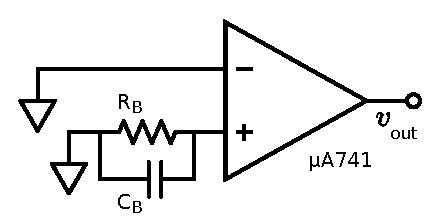
\includegraphics[width=0.40\textwidth]{../E02/latex/direct_measure.pdf}
  \end{center}
  \caption{Schema del circuito utilizzato per stimare la corrente di polarizzazione. La resistenza utilizzata è di $10.36\pm0.01$\si{\mega\ohm}; la capacità $102 \pm 1$ \si{\nano\farad}.}
  \label{gen_continua}
\end{wrapfigure}

Nel circuito mostrato in figura abbiamo posto la resistenza all'ingresso non invertente (analogamente si può fare con l'ingresso invertente) e, misurando la caduta di potenziale ai capi della stessa con il multimetro, possiamo ottenere il valore di corrente desiderato applicando semplicemente la legge di Ohm

$$V=I_{b^+} R$$

Per far ciò, dato che attendevamo una corrente dell'ordine dei \si{\nano\ampere}, abbiamo utilizzato una resistenza molto grande in modo da poter leggere il valore della tensione su una scala accettabile per il multimetro.

Durante la procedura abbiamo però notato che, a causa di rumori ambientali, il valore di tensione sul multimetro fluttuava sulla prima cifra, rendendo nostra misurazione ovviamente non quantitativa (al massimo poteva stimarci l'ordine di grandezza della corrente). Per ovviare, abbiamo inserito in parallelo alla resistenza un condensatore che caricandosi si portava alla stessa ddp dei capi della resistenza. In questo modo abbiamo potuto ottenere un valore meno fluttuante, che si attestava a $V=(-80 \pm 2)$ \si{\milli\volt}, cioè $I_{b^+}=(7.7 \pm 0.2)$ \si{\nano\ampere}.

Con questo metodo semplice abbiamo potuto ottenere una prima stima del valore della corrente. Di contro bisogno considerare che il rumore non permette di avere una stima qualitativa ed inoltre la resistenza, scaldandosi, modifica il suo valore e potrebbe portare ad un errore sulla misura. Nel paragrafo successivo progetteremo dunque un circuito che, sfruttando l'amplificazione data dall'amplificatore operazionale, minimizzerà questi errori.

\subsection{Configurazione con retroazione negativa}

Sfruttando un modello simile a quello utilizzato per trovare la tensione di offset, abbiamo montato i circuiti come in figura.

\subsubsection{Misura di $I_{b^-}$}

Risolviamo il circuito per trovare la corrente di polarizzazione $I_{b^-}$ in funzione della tensione di uscita. Considerando $V_{-}$ la tensione al capo di $R_B$ collegato all'OPAMP e $V^*$ quello opposto, vale in quel punto la legge di Kirchhoff sui nodi

$$\frac{V^* - V_{in}}{R_1} + \frac{V^*-V_{out}}{R_2} + \frac{V^*-V_{-}}{R_B}=0$$

Dato che l'amplificatore operazionale è considerato già stabilizzato per quanto riguarda la tensione di offset, possiamo considerare la tensione all'ingresso invertente uguale all'ingresso non invertente. Vale dunque che $V_{in}=V_{-}=0$ e si trova (considerando $I_{b^-} R_B = V^*$:

$$I_{b^-}=\frac{V_{out}}{R_2}\frac{1}{\frac{1}{R_1}+\frac{1}{R_2}+\frac{1}{R_B}}$$

La misura di tensione di uscita è di $-362.7$ \si{\milli\volt} ed il valore ottenuto è dunque $I_{b^-} = (3.62 \pm 0.02)$ \si{\nano\ampere}.

\subsubsection{Misura di $I_{b^-}$}

Similmente a quanto visto per la configurazione prima, troviamo che, data la legge di Kirchhoff

$$\frac{V^* - V_{in}}{R_1} + \frac{V^*-V_{out}}{R_2} + \frac{V^*-V_{-}}{R_B}=0$$

e con considerazioni analoghe al paragrafo precedente

$$I_{b^-}=\frac{V_{out}}{R_2 R_B}\frac{1}{\frac{1}{R_1}+\frac{1}{R_2}}$$

La misura di tensione di uscita è di $370.3$ \si{\milli\volt} ed il valore ottenuto è dunque $I_{b^+} = (3.70 \pm 0.03)$ \si{\nano\ampere}.
\subsection{Conclusioni}
In questa esperienza abbiamo potuto osservare come gli OPAMP, sebbene siano dei circuiti abbastanza precisi, abbiano delle imperfezioni, date dalla loro composizione circuitale (sono presenti dei transistor BJT al loro interno).
Le discrepanze tra il modello ideale e l'OPAMP reale sono date principalmente dallo sbilanciamento della risposta dello stesso ($V_{offset}$) e dalle correnti di polarizzazione (\textit{bias currents}).
Per nostra fortuna spesso gli OPAMP presentano dei connettori predisposti a minimizzare la tensione di offset con circuiti di compensazione: nel nostro caso un trigger collegato ai piedini di offset e all'alimentazione negativa.
Una volta bilanciato l'opamp, abbiamo misurato le correnti di polarizzazione e abbiamo potuto osservare che esse sono dell'ordine dei \si{\nano\ampere}, quindi trascurabili per gli utilizzi più comuni.



\end{document}